% !TeX program = XeLaTeX or LuaLaTeX
% !TeX encoding = UTF-8 Unicode
\documentclass[a4paper,oneside,12pt]{article}
%%%%%%%%%%%%%%%%%%%%%%%%%%%%%%%%%%%%%%%%%%%%%%%%%%%%%%%%%%%%%%%%%%%%%%%%%%%%%%%%%
%% Packages
%%%%%%%%%%%%%%%%%%%%%%%%%%%%%%%%%%%%%%%%%%%%%%%%%%%%%%%%%%%%%%%%%%%%%%%%%%%%%%%%%
\usepackage[spanish]{babel}
% \usepackage[ddmmyyyy]{datetime}
\usepackage{multirow}
\usepackage{amsmath}
\usepackage{fontspec}
% \usepackage{complexity}
% \usepackage[T1]{fontenc}
% \usepackage[utf8]{inputenc}
% \usepackage[pdftex]{graphicx} %%Graphics in pdfLaTeX
\usepackage[xetex]{graphicx}
\usepackage{csquotes}
\usepackage{a4wide} %%Smaller margins, more text per page.
\usepackage{longtable} %%For tables that exceed a page width
\usepackage{pdflscape} %%Adds PDF sup­port to the land­scape en­vi­ron­ment of pack­age
\usepackage{caption} %%Pro­vides many ways to cus­tomise the cap­tions in float­ing en­vi­ron­ments like fig­ure and ta­ble
\usepackage{float} %%Im­proves the in­ter­face for defin­ing float­ing ob­jects such as fig­ures and ta­bles
\usepackage[tablegrid,nochapter]{vhistory} %%Vhis­tory sim­pli­fies the cre­ation of a his­tory of ver­sions of a doc­u­ment
\usepackage[nottoc]{tocbibind} %%Au­to­mat­i­cally adds the bib­li­og­ra­phy and/or the in­dex and/or the con­tents, etc., to the Ta­ble of Con­tents list­ing
\usepackage[toc,page]{appendix} %%The ap­pendix pack­age pro­vides var­i­ous ways of for­mat­ting the ti­tles of ap­pen­dices
\usepackage{pdfpages} %%This pack­age sim­pli­fies the in­clu­sion of ex­ter­nal multi-page PDF doc­u­ments in LATEX doc­u­ments
\usepackage[rightcaption]{sidecap} %%De­fines en­vi­ron­ments called SC­fig­ure and SCtable (anal­o­gous to fig­ure and ta­ble) to type­set cap­tions side­ways
% \usepackage{cite} %%The pack­age sup­ports com­pressed, sorted lists of nu­mer­i­cal ci­ta­tions, and also deals with var­i­ous punc­tu­a­tion and other is­sues of rep­re­sen­ta­tion, in­clud­ing com­pre­hen­sive man­age­ment of break points
\usepackage[printonlyused]{acronym} %%This pack­age en­sures that all acronyms used in the text are spelled out in full at least once. It also pro­vides an en­vi­ron­ment to build a list of acronyms used
% \usepackage[pdftex,scale={.8,.8}]{geometry} %%The pack­age pro­vides an easy and flex­i­ble user in­ter­face to cus­tomize page lay­out, im­ple­ment­ing auto-cen­ter­ing and auto-bal­anc­ing mech­a­nisms so that the users have only to give the least de­scrip­tion for the page lay­out. For ex­am­ple, if you want to set each mar­gin 2cm with­out header space, what you need is just \usep­a­ck­age[mar­gin=2cm,no­head]{ge­om­e­try}.
\usepackage{layout} %%The pack­age de­fines a com­mand \lay­out, which will show a sum­mary of the lay­out of the cur­rent doc­u­ment
\usepackage{subfigure} %%Pro­vides sup­port for the ma­nip­u­la­tion and ref­er­ence of small or ‘sub’ fig­ures and ta­bles within a sin­gle fig­ure or ta­ble en­vi­ron­ment.
\usepackage[toc]{glossaries} %%The glos­saries pack­age sup­ports acronyms and mul­ti­ple glos­saries, and has pro­vi­sion for op­er­a­tion in sev­eral lan­guages (us­ing the fa­cil­i­ties of ei­ther ba­bel or poly­glos­sia).
\usepackage[left,pagewise,modulo]{lineno} %%Adds line num­bers to se­lected para­graphs with ref­er­ence pos­si­ble through the LATEX \ref and \pageref cross ref­er­ence mech­a­nism
\usepackage[xetex,colorlinks=false,hidelinks,pdfstartview=FitV,bookmarks=true]{hyperref}%%The hy­per­ref pack­age is used to han­dle cross-ref­er­enc­ing com­mands in LATEX to pro­duce hy­per­text links in the doc­u­ment. 
\usepackage{metainfo}
\usepackage[top=1in,bottom=1in,left=1in,right=1in]{geometry}
% \usepackage[a4paper,left=2.5cm,right=2.5cm,top=\dimexpr15mm+1.5\baselineskip,bottom=2cm]{geometry}
\usepackage{geometry}
% \usepackage[pagestyles,raggedright]{titlesec}
\usepackage{etoolbox}
\usepackage{tabularx}
\usepackage{ltxtable}
\usepackage[style=ieee]{biblatex}
\bibliography{CD.bib}
\usepackage[nottoc]{tocbibind}
\usepackage[official]{eurosym}
\usepackage{gensymb}
\usepackage{qrcode}
\usepackage{numprint}
\usepackage{mathtools}
\usepackage[nice]{nicefrac}
\usepackage{tikz}
\usetikzlibrary{arrows,automata,babel,positioning}
\usepackage{%
    array, %%An ex­tended im­ple­men­ta­tion of the ar­ray and tab­u­lar en­vi­ron­ments which ex­tends the op­tions for col­umn for­mats, and pro­vides "pro­grammable" for­mat spec­i­fi­ca­tions
    booktabs, %%The pack­age en­hances the qual­ity of ta­bles in LATEX, pro­vid­ing ex­tra com­mands as well as be­hind-the-scenes op­ti­mi­sa­tion
    dcolumn, %%
    rotating,
    shortvrb,
    units,
    url,
    lastpage,
    longtable,
    lscape,
    qtree,
    skmath,	
    enumitem,
    wasysym,
    mathcomp,
    titling,
    % libertineotf,
    libertine,
    fancyhdr,
}

\newcommand{\bigO}[1]{%
  \text{\usefont{OMS}{cmsy}{m}{n}O}\left(#1\right)%
}
%%%%%%%%%%%%%%%%%%%%%%%%%%%%%%%%%%%%%%%%%%%%%%%%%%%%%%%%%%%%%%%%%%%%%%%%%%%%%%%%%
%% Java --> latex 
%%%%%%%%%%%%%%%%%%%%%%%%%%%%%%%%%%%%%%%%%%%%%%%%%%%%%%%%%%%%%%%%%%%%%%%%%%%%%%%%%
\setmonofont{Fira Code}[
  Contextuals=Alternate,
  Ligatures = {Common,Rare}
]
\usepackage{letltxmacro}
\LetLtxMacro\oldttfamily\ttfamily
\DeclareRobustCommand{\ttfamily}{\oldttfamily\csname ttsize\endcsname}
\newcommand{\settttsize}[1]{\def\ttsize{#1}}%
\usepackage{lstfiracode}
\usepackage{listings}

\lstset{ %
  backgroundcolor=\color{white},   % Indica el color de fondo; necesita que se añada \usepackage{color} o \usepackage{xcolor}
  basicstyle=\footnotesize\ttfamily,        % Fija el tamaño del tipo de letra utilizado para el código
  breakatwhitespace=false,         % Activarlo para que los saltos automáticos solo se apliquen en los espacios en blanco
  inputencoding=utf8,
  breaklines=true,                 % Activa el salto de línea automático
  captionpos=b,                    % Establece la posición de la leyenda del cuadro de código
  commentstyle=\color{darkgreen},    % Estilo de los comentarios
  extendedchars=true,              % Permite utilizar caracteres extendidos no-ASCII; solo funciona para codificaciones de 8-bits; para UTF-8 no funciona. En xelatex necesita estar a true para que funcione.
  frame=single,	                   % Añade un marco al código
  keepspaces=true,                 % Mantiene los espacios en el texto. Es útil para mantener la indentación del código(puede necesitar columns=flexible).
  columns=flexible,
  keywordstyle=\color{darkorange},       % estilo de las palabras clave
  numbers=left,                    % Posición de los números de línea (none, left, right).
  numbersep=5pt,                   % Distancia de los números de línea al código
  numberstyle=\small\color{gray}, % Estilo para los números de línea
  rulecolor=\color{black},         % Si no se activa, el color del marco puede cambiar en los saltos de línea entre textos que sea de otro color, por ejemplo, los comentarios, que están en verde en este ejemplo
  showspaces=false,                % Si se activa, muestra los espacios con guiones bajos; sustituye a 'showstringspaces'
  showstringspaces=false,          % subraya solamente los espacios que estén en una cadena de esto
  showtabs=false,                  % muestra las tabulaciones que existan en cadenas de texto con guión bajo
  stringstyle=\color{darkgreen},     % Estilo de las cadenas de texto
  style=FiraCodeStyle,
  identifierstyle=\color{blue},
  tabsize=4,	                   % Establece el salto de las tabulaciones a 2 espacios
  title=\lstname,                   % muestra el nombre de los ficheros incluidos al utilizar
  caption=\lstname,
  literate={á}{{\'a}}1 {é}{{\'e}}1 {í}{{\'{\i}}}1 {ó}{{\'o}}1 {ú}{{\'u}}1 {Á}{{\'A}}1 {É}{{\'E}}1 {Í}{{\'I}}1 {Ó}{{\'O}}1 {Ú}{{\'U}}1 {ü}{{\"u}}1 {Ü}{{\"U}}1 {ñ}{{\~n}}1 {Ñ}{{\~N}}1 {¿}{{?``}}1 {¡}{{!``}}1 {º}{\textdegree}1,
  postbreak=\mbox{\textcolor{red}{$\hookrightarrow$}\space},
  linewidth=1.1\linewidth
}
\lstdefinestyle{C}{%
  language=C,                 % El lenguaje del código
  otherkeywords={__attribute__, __interrupt__, inline, asm, uint8_t, uint16_t,%
  uint32_t, uint64_t, time_t, size_t, servo_t, motor_t, Nop,%
  point_t, angle_t, double64_t, int_fast64_t, bool, true, false, stdbool, stdint,%
  stdlib, stddef, NULL}           % Si se quieren añadir otras palabras clave al lenguaje
}
\lstdefinestyle{Python}{%
  language=Python
}

\lstdefinestyle{Ada}{%
  language=Ada
}
\lstdefinestyle{bash}{%
  language=bash,
  otherkeywords={sudo,chmod,chown,chgrp,ls,mkdir,touch,useradd,groupadd,usermod}
}
\lstdefinestyle{R}{%
  language=R,
  otherkeywords={0,1,2,3,4,5,6,7,8,9},
  morekeywords={TRUE,FALSE},
  deletekeywords={data,frame,length,as,character,time,ts}
}
\usepackage{xcolor}
\definecolor{pblue}{rgb}{0.13,0.13,1}
\definecolor{pgreen}{rgb}{0,0.5,0}
\definecolor{pred}{rgb}{0.9,0,0}
\definecolor{pgrey}{rgb}{0.46,0.45,0.48}
\definecolor{darkgreen}{rgb}{0.0, 0.4, 0.0}
\definecolor{darkorange}{rgb}{1.0, 0.55, 0.0}
% \usepackage{inconsolata}
%%%%%%%%%%%%%%%%%%%%%%%%%%%%%%%%%%%%%%%%%%%%%%%%%%%%%%%%%%%%%%%%%%%%%%%%%%%%%%%%%
% \setlength{\parindent}{0pt}
\setlength{\parskip}{.5\baselineskip}
%% Checkmark symbols
\usepackage{pifont}
\newcommand{\cmark}{\ding{51}}%
\newcommand{\xmark}{\ding{55}}%
\newcommand{\done}{\rlap{$\square$}{\raisebox{2pt}{\large\hspace{1pt}\cmark}}%
\hspace{-2.5pt}}
\newcommand{\wontfix}{\rlap{$\square$}{\large\hspace{1pt}\xmark}}
%%%%%%%%%%%%%%%%%%%%%%%%%%%%%%%%%%%%%%%%%%%%%%%%%%%%%%%%%%%%%%%%%%%%%%%%%%%%%%%%%
%% Creation of the header
%%%%%%%%%%%%%%%%%%%%%%%%%%%%%%%%%%%%%%%%%%%%%%%%%%%%%%%%%%%%%%%%%%%%%%%%%%%%%%%%%
\patchcmd{\chapter}{plain}{short}{}{} %$ <-- the header on chapter 1
% % workaround
% \makeatletter
% \appto{\appendices}{\def\Hy@chapapp{Appendix}}
% \makeatother
\addto\captionsspanish{%
  \renewcommand\appendixname{Anexo}
  \renewcommand\appendixpagename{Anexos}
}
\newcolumntype{s}{>{\hsize=.5\hsize\linewidth=\hsize}X}
\newcolumntype{b}{>{\hsize=.75\hsize}X}
\newcommand{\heading}[1]{\multicolumn{1}{c}{#1}}
\newcolumntype{L}[1]{>{\hsize=#1\hsize\raggedright\arraybackslash}X}%
\newcolumntype{R}[1]{>{\hsize=#1\hsize\raggedleft\arraybackslash}X}%
\newcolumntype{C}[1]{>{\hsize=#1\hsize\centering\arraybackslash}X}%

% \usepackage[definemenumacros=false]{menukeys}

\DeclareMathOperator{\atantwo}{atan2}

\DeclareMathOperator{\arctantwo}{arctan2}
%%%%%%%%%%%%%%%%%%%%%%%%%%%%%%%%%%%%%%%%%%%%%%%%%%%%%%%%%%%%%%%%%%%%%%%%%%%%%%%%%
%% DOCUMENT
%%%%%%%%%%%%%%%%%%%%%%%%%%%%%%%%%%%%%%%%%%%%%%%%%%%%%%%%%%%%%%%%%%%%%%%%%%%%%%%%%
\author{Javier Alonso Silva\\Alfonso Díez Ramírez\\Sara Moreno Prieto\\Mihai Octavian St\u{a}nescu}
\title{STRD -- Detección de distracciones al volante}
\date{2021}
% \setlength{\droptitle}{-4cm}
\pagestyle{fancy}
\fancyhf{}
\fancyhfoffset[L]{1cm} % left extra length
\fancyhfoffset[R]{1cm} % right extra length
\rhead{2021}
\chead{\thetitle}
\lhead{\slshape\nouppercase{\leftmark}}
\cfoot{\thepage}
\pagenumbering{roman}

\begin{document}
\settttsize{\footnotesize}
\ActivateVerbatimLigatures
\maketitle
\begin{abstract}
    Se desarrolla un sistema de detección de distracciones al volante el
    cual se espera ayude a evitar los posibles accidentes derivados de
    la casuística anterior.

    El desarrollo consiste en una evaluación de los requisitos, modelado del
    sistema mediante diagramas SysML hasta una implementación final en dos
    nodos diferenciados los cuales se comunican entre sí usando la tecnología
    CANBus.

    El primer nodo (\textit{nodo 1}) tendrá una carga balanceada entre la lectura
    de dispositivos así como la intervención en elementos físicos del vehículo,
    como son los frenos; y a su vez será el encargado de una transmisión continua
    de mensajes hacia el segundo nodo. El \textit{nodo 2} leerá información sobre
    el estado psico-físico del conductor y, junto con la información recibida del
    \textit{nodo 1}, alertará al mismo sobre distintos factores que se han visto
    peligrosos para que pueda reconducir su comportamiento. Finalmente, se ofrece
    al conductor un método para evitar ser distraído por el propio sistema pudiendo
    decidir entre tres niveles de avisos: completo, parcial e inactivo.
\end{abstract}
%
\rule{\linewidth}{.2pt}
\newpage
\tableofcontents
\newpage

\pagenumbering{arabic}

\section{Introducción}
Una de las mayores causas de accidentes son las distracciones de los conductores
al volante, o bien por el uso de dispositivos electrónicos, somnolencia u otras
acciones que llevan a la persona a no prestar atención a la carretera y su entorno.

A raíz de ese problema, los mecanismos de regulación internacionales han invertido
tiempo, dinero y desarrollo en los sistemas ADAS (\textit{Advanced Driving Assistance Systems}),
con el fin de mitigar las situaciones anteriores y realizar una prevención activa
sobre los accidentes de tráfico. Sin embargo, dichos sistemas no cuentan con una
penetración significativa en el mercado, por lo que interesa agilizar su implantación
y que pasen a ser un elemento de seguridad ``por defecto'' en los nuevos vehículos.

En este contexto, se ha pedido realizar una implementación distribuida, que cumpla con
unos requisitos de tiempo real, en dos nodos que interactúan entre sí para actuar
como un organismo conjunto sobre un vehículo como sistema ADAS.

El sistema a desarrollar contará con múltiples sensores:
\begin{itemize}
  \item Giroscopio, para detectar en los ejes $X$ y $Y$ la inclinación de la cabeza
        del conductor y predecir una posible somnolencia.
  \item Giro del volante, para detectar si el conductor está pegando volantazos o está
        realizando ``mini--correcciones'', características de un estado de somnolencia o
        de atender al móvil.
  \item Agarre del volante, donde se indicará si el conductor está agarrando el volante
        o no.
  \item Velocímetro, con un rango de valores comprendido entre los
        $\left[0, 200\right] \nicefrac{km}{h}$. Se usará para comprobar que se cumple
        la distancia de seguridad.
  \item Sensor de distancia, capaz de realizar lecturas en el rango $\left[5, 200\right]~m$
        y que le indicará al conductor si está cumpliendo o no la distancia de seguridad,
        según la velocidad a la que circule.
\end{itemize}

y múltiples actuadores:
\begin{itemize}
  \item Luces de aviso, las cuales se usarán para emitir señales luminosas al conductor
        indicando cierto nivel de riesgo que se está produciendo.
  \item \textit{Display}, usado para visualizar los datos que obtiene el sistema.
  \item Alarma sonora, emitiendo un sonido con 3 niveles de intensidad.
  \item Luz de aviso/freno automático, donde ante un peligro de colisión inminente
        el sistema podrá activar el freno con hasta 3 niveles de intensidad.
\end{itemize}

Cada uno de los sensores/actuadores estarán controlados y monitorizados por una o
varias tareas las cuales registran los datos en objectos protegidos. Dichas tareas
vienen definidas con sus periodos y \textit{deadlines} en el cuadro \ref{tab:tasks}:

\begin{table}[H]
  \centering
  \begin{tabularx}{\linewidth}{C{.3}|c|c|c|c|c|c|c}
    \textbf{Tareas/objetos protegidos} & \textbf{Tipo} & $T_i$  & $D_i$  & \textbf{WCET} & \textbf{Síntomas 1} & \textbf{Síntomas 2} & \textbf{Modo} \\
    \hline
    Inclinación cabeza                 & C             & $600$  & $400$  & ?             & $x_1$               &                     &               \\
    Detección de volantazos            & C             & $400$  & $400$  & ?             & $x_1$               &                     &               \\
    Cálculo distancia                  & C             & $300$  & $300$  & ?             &                     & $y_1$               &               \\
    Relax al volante                   & C             & $500$  & $200$  & ?             & $x_1$               &                     &               \\
    Emergencias                        & C             & $300$  & $300$  & ?             & $x_2$               & $y_2$               & $z_2$         \\
    Mostrar información                & C             & $2000$ & $2000$ & ?             & $x_2$               & $y_2$               &               \\
    Detección pulsador                 & S             & -      & $100$  & ?             &                     &                     & $z_1$         \\
    \hline\hline
    Síntomas 1                         & P             & -      & -      & $x_1, x_2$    &                     &                     &               \\
    Síntomas 2                         & P             & -      & -      & $y_1, y_2$    &                     &                     &               \\
    Modo                               & P             & -      & -      & $z_1, z_2$    &                     &                     &               \\
    \hline\hline
  \end{tabularx}
  \caption{Listado de tareas y objetos protegidos junto con sus tiempos.}
  \label{tab:tasks}
\end{table}

Como hay multitud de tareas y se cuenta con dos nodos, el sistema a implementar irá
distribuído entre ambos y viene representado por la figura \ref{fig:system-full}:

\begin{figure}[H]
  \centering
  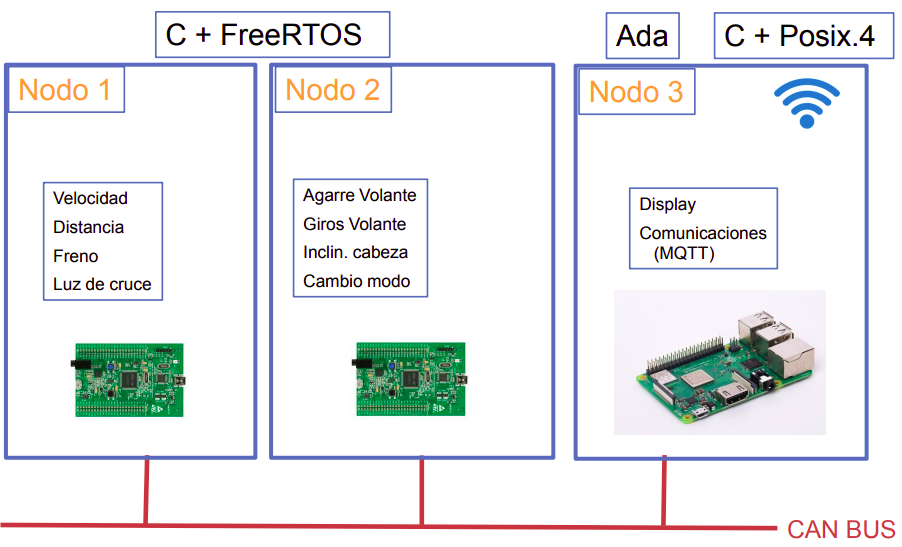
\includegraphics[width=.7\linewidth]{pictures/system-full.png}
  \caption{Modelo completo del sistema a implementar. Las tareas van distribuídas entre
    los dos nodos principales y se comunican entre ellos mediante CANBus.}
  \label{fig:system-full}
\end{figure}

\subsection{Nodo 1}
El primer nodo será el encargado principalmente de la actuación sobre distintos
elementos del sistema, a saber: el freno, las luces de cruce e indirectamente sobre
la alarma. Esto lo hará recogiendo datos de distintos sensores como son el velocímetro,
el sensor de distancia y el sensor de luminosidad para adecuar su comportamiento a las
circunstancias del entorno.

Este sistema contará con cuatro tareas en tiempo real y usará dos objetos protegidos:
el primero de ellos para conservar el valor de la velocidad actual; y el segundo para
guardar tanto el valor de la distancia con el vehículo precedente como la intensidad
del freno que se ha de aplicar en caso de peligro de colisión. Por su parte, las
tareas en cuestión son:

\begin{enumerate}
  \item \texttt{Cálculo velocidad} -- cada $\numprint[ms]{250}$, realizará una lectura
        del sensor en cuestión mediante el ADC y actualizará el valor del objeto 
        protegido \texttt{V\_actual}.
  \item \texttt{Cálculo distancia} -- cada $\numprint[ms]{300}$, el sistema obtendrá la
        distancia con el vehículo precedente usando el sensor de ultrasonidos y
        actualizará el valor del objeto protegido \texttt{D\_actual}. Además, leerá el
        valor de \texttt{V\_actual} y computará lo que sería la distancia de seguridad
        mínima que hay que respetar, descrita por la ecuación \ref{eq:min-dist}:

        \begin{equation}\label{eq:min-dist}
          d_{\min} = \left(\frac{V}{10}\right)^2,~\begin{cases}
            d_{\min} &: \text{distancia mínima que hay que mantener.} \\
            V &: \text{velocidad actual del vehículo.}
          \end{cases}
        \end{equation}

        En caso de que la distancia de seguridad no se cumpla (y según el valor relativo
        con que no se cumple), la tarea indicará en \texttt{Intens\_Frenada} con qué
        intensidad se ha de aplicar el freno para evitar una colisión. Finalmente,
        activará la tarea esporádica \texttt{Freno} para que realice su ejecución.
  \item \texttt{Freno} -- cada $\numprint[ms]{150}$ como mucho, realizará la activación
        progresiva del freno cada $\numprint[ms]{100}$ hasta alcanzar la intensidad
        apropiada. Al ser una tarea esporádica, depende directamente de la activación
        desde \texttt{Cálculo distancia}, lo cual añadirá un \textit{jitter} al tiempo
        de respuesta global de la tarea.
  \item \texttt{Luces de cruce} -- cada $\numprint[ms]{1000}$, el sistema realizará una
        valoración de la luminosidad del entorno y procederá a encender o apagar automáticamente
        las luces de cruce. Se establece que las luces se activarán si la intensidad lumínica
        está por debajo de $100$.
\end{enumerate}

Todo este sistema viene modelado por la figura \ref{fig:node1}:

\begin{figure}[H]
  \centering
  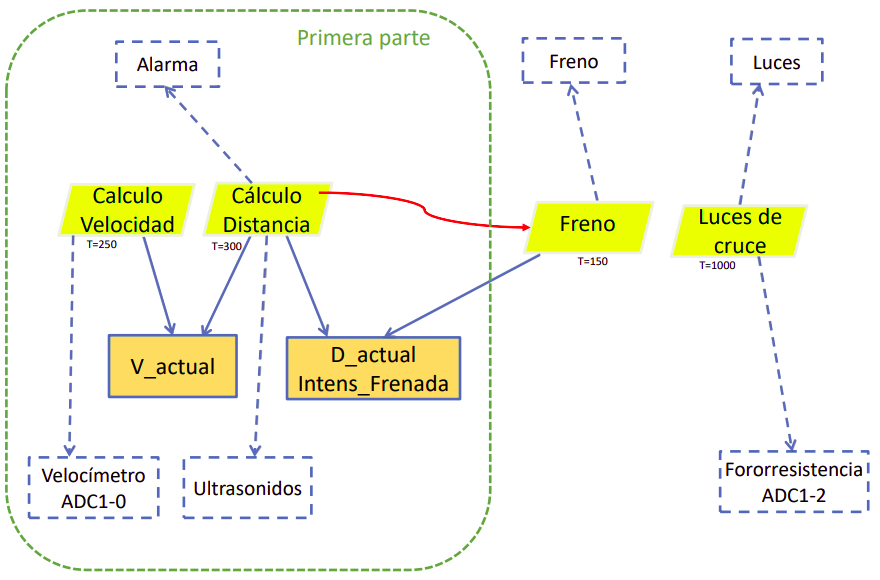
\includegraphics[width=.8\linewidth]{pictures/node1.png}
  \caption{Modelado del nodo 1 junto con sus tareas, objetos protegidos, sensores y actuadores.}
  \label{fig:node1}
\end{figure}

\subsection{Nodo 2}
El segundo nodo se encargará directamente de notificar al conductor cuando algún
comportamiento es errático o peligroso. Entre otras tareas, este nodo se encarga
de monitorizar el estado del conductor (y detectar posibles signos de somnolencia)
y emitir avisos luminosos y sonoros cuando se produzcan situaciones de riesgo.

Este sistema cuenta con cinco tareas en tiempo real y tres objetos protegidos: el
primero recoge datos sobre síntomas como son la inclinación de la cabeza o el
giro del volante; el segundo, recoge información sobre si el conductor está
sujetando o no el volante; y el tercero establecerá el modo de funcionamiento de
los avisos del sistema. Con respecto a las tareas, se tiene:

\begin{enumerate}
  \item \texttt{Inclinación cabeza} -- cada $\numprint[ms]{600}$, leerá el valor del
        giroscopio integrado para actualizar los datos de las posiciones $X$ e $Y$,
        en el objeto protegido \texttt{Síntomas 1}.
  \item \texttt{Detección volantazos} -- cada $\numprint[ms]{400}$ el sistema leerá
        el valor de la posición del volante y actualizará el dato recogido en 
        \texttt{Síntomas 1}.
  \item \texttt{Relax al volante} -- cada $\numprint[ms]{500}$, el sistema actualizará
        en \texttt{Síntomas 2} si el conductor está sujetando o no el volante.
  \item \texttt{Detección pulsador} -- tarea esporádica que será activada desde la rutina
        de tratamiento de interrupciones \textit{hardware} que establecerá cíclicamente
        el modo de funcionamiento del sistema en el objeto protegido \texttt{Modo}.
  \item \texttt{Riesgos} -- cada $\numprint[ms]{300}$, el sistema evaluará los datos
        recogidos en los objetos protegidos \texttt{Síntomas 1}, \texttt{Síntomas 2} y \texttt{Modo} y 
        establecerá el nivel de alarma para con el conductor. Dicha detección de riesgos
        viene definida por la siguiente secuencia:
        \begin{itemize}
          \item Si el conductor presenta una inclinación de la cabeza en los ejes $X, Y$
                de más de $20\degree$ y no tiene sujeto el volante se considera que está
                manipulando el móvil u otro aparato. Se activa la luz amarilla y se
                emite un pitido nivel 1.
          \item Si la inclinación de la cabeza es $X > 20\degree | Y > 20\degree$, el volante
                está agarrado y la velocidad es mayor de $70\nicefrac{km}{h}$ se interpreta
                que el conductor no está prestando atención a la carretera y se encenderá la
                luz amarilla.
          \item Si se detecta una inclinación en el eje $X$ de más de $30\degree$ y el
                conductor está dando volantazos se interpreta como síntoma de somnolencia.
                Se encenderá la luz amarilla y se emitirá un pitido nivel 2.
          \item Si se dan simultáneamente dos de los riegos anteriores se pasa a estar en 
                \textbf{NIVEL 2} de alerta y se encenderá la luz roja y emitirá un pitido
                nivel 2.
          \item Si se produce un riesgo \textbf{NIVEL 2} y la distancia con el vehículo
                precedente es menor al 50\% de la distancia de seguridad recomendada, se
                estará ante una situación de \textbf{EMERGENCIA} y se activará el freno, 
                junto con todo lo anterior.
        \end{itemize}
\end{enumerate}

\section{Implementación}
Una vez se ha introducido el sistema, se va a explicar la implementación
que se ha realizado finalmente en cada uno de los nodos. Como esta memoria es de
explicación del código y de las decisiones tomadas, se incluirán distintos fragmentos
del mismo para acompañar a las explicaciones y entrar en mayor o menor detalle
en las funciones.

Por otra parte, se va a explicar qué tareas se han implementado correctamente en cada
uno de los nodos y cómo se han implementado.

Finalmente, destacar que hay fragmentos de código fuente que son comunes a ambos nodos
y que no aparecerán explicados en detalle por cada nodo sino que se indican en el anexo
\ref{anx:common-code}.
\subsection{Nodo 1}
En el nodo 1 se han implementado en principio todas las tareas cumpliendo con las
restricciones pedidas.

La tarea del \texttt{Cálculo de velocidad} viene definida por el listado de código
\ref{lst:speedtask}:

\lstinputlisting[style=C,caption={Tarea periódica que controla el acelerador.},label={lst:speedtask},linerange={90-114},firstnumber=90]{source-code/node1/Src/main.c}

En la susodicha tarea se lee el ADC desde el canal 0 y el valor recibido de la velocidad
se mapea de $0$ a $200 \nicefrac{km}{h}$ (línea 108). A continuación, se actualiza el valor del
objeto protegido (línea 109) y se envía el dato recibido por el CANBus (línea 110).
Finalmente, se programa la siguiente ejecución dentro de $\numprint[ms]{250}$ desde el
instante de activación (línea 112).

La función de \texttt{map} viene definida en los códigos \ref{lst:utils_h} y \ref{lst:utils_c}.
El objeto protegido \texttt{SPEED} sigue la definición estándar del resto de objetos
protegidos y viene definido en los códigos \ref{lst:speed_h} (cabeceras) y \ref{lst:speed_c}
(cuerpo).

Por otra parte, el envío de datos mediante el CANBus se realiza mediante la librería
\texttt{can}, definida en los códigos \ref{lst:can_h} y \ref{lst:can_c}.

La tarea del \texttt{Cálculo distancia} viene definida por el código \ref{lst:distancetask}:

\lstinputlisting[style=C,caption={Tarea periódica que controla la distancia.},label={lst:distancetask},linerange={116-165},firstnumber=116]{source-code/node1/Src/main.c}

En dicha tarea se utiliza la librería \texttt{uss} (códigos \ref{lst:uss_h} y \ref{lst:uss_c})
para leer desde el sensor de ultrasonidos (líneas 135 -- 137); se actualiza el valor de la distancia en el
objeto protegido \texttt{distance} (línea 138) (códigos \ref{lst:distance_h} y \ref{lst:distance_c});
se computa la distancia de seguridad y se calcula la intensidad de la frenada
según unos porcentajes establecidos (líneas 140 -- 156); si el valor de la intensidad de
la frenada ha cambiado, se actualiza el objeto protegido y se notifica a la tarea
esporádica que puede continuar su ejecución (líneas 158 -- 161) 
(códigos \ref{lst:brake_h} y \ref{lst:brake_c}); finalmente, se
envía el valor de la nueva distancia por el CANBus (línea 162) y se programa la
siguiente ejecución $\numprint[ms]{300}$ después del instante de activación (línea 163).

La tarea esporádica \texttt{Freno} viene definida por el código \ref{lst:braketask}:

\lstinputlisting[style=C,caption={Tarea esporádica que controla la intensidad de la frenada.},label={lst:braketask},linerange={167-224},firstnumber=167]{source-code/node1/Src/main.c}

Dicha tarea espera a que se le notifique que se ha de ejecutar (línea 180) y después accede
al objeto protegido que contiene la intensidad de la frenada (códigos \ref{lst:distance_h} y
\ref{lst:distance_c}); a continuación, según la intensidad de la frenada, enciende o
apaga diversos LEDs en la placa a modo de indicativo visual de que se está frenando
(líneas 183 -- 220). Finalmente, para evitar que la tarea se pueda activar con una
baja periodicidad se esperan al menos $\numprint[ms]{150}$ desde el instante de activación.

Finalmente, la tarea de gestión de las \texttt{Luces de cruce} viene definida por el código
\ref{lst:lightstask}:

\lstinputlisting[style=C,caption={Tarea periódica que controla las luces de cruce.},label={lst:lightstask},linerange={226-251},firstnumber=226]{source-code/node1/Src/main.c}

Dicha tarea lee desde el ADC (canal 1) el valor recibido por el LDR y, tras comprobar
su luminosidad con el rango establecido enciende o apaga las luces de cruce (líneas 245 -- 247).
Finalmente, se programa la siguiente ejecución $\numprint[s]{1}$ después de la
activación. Esta tarea no accede a ningún objeto protegido.\\
\rule{\linewidth}{.2pt}

Cabe destacar que los distintos objetos protegidos que se declaran y usan a lo largo
del código se basan en la librería \texttt{lock}, definida en los códigos \ref{lst:lock_h}
y \ref{lst:lock_c}. Dicha librería requiere que los objetos protegidos sean inicializados
antes de realizar ninguna operación con ellos. Por ende, en el bloque \texttt{main} es
necesario dedicar unas líneas para iniciar cada una de los objetos protegidos que se
quieren usar (código \ref{lst:main_init1}):

\lstinputlisting[style=C,caption={Código del \texttt{main}.},label={lst:main_init1},linerange={253-300},firstnumber=253]{source-code/node1/Src/main.c}

En las líneas 271 -- 274 se inicializan los objetos protegidos, dejándolos listos para su
uso. El cuerpo viene definido en los códigos \ref{lst:can_c}, \ref{lst:speed_c},
\ref{lst:distance_c}, \ref{lst:brake_c}.

\subsection{Nodo 2}
En el nodo 2 se han implementado también todas las tareas y requisitos pedidos
en el documento de requisitos.

La tarea de actualización del modo de funcionamiento viene definida por el código
\ref{lst:modetask}:

\lstinputlisting[style=C,caption={Tarea esporádica que controla el modo.},label={lst:modetask},linerange={110-124},firstnumber=110]{source-code/node2/Src/main.c}

Dicha tarea espera a un semáforo binario que indica que se ha producido una interrupción
(línea 119). Una vez desbloqueada, incrementa el modo hasta un máximo de `2' (línea 120)
y finalmente actualiza el objeto protegido \texttt{mode} (códigos \ref{lst:mode_h} y
\ref{lst:mode_c}).

Por otra parte, como hace falta liberar el semáforo cuando se produce la interrupción
del pulsador, es necesario definir un nuevo fragmento del código que habilite a la
placa para esa tarea (código \ref{lst:exti}):

\lstinputlisting[style=C,caption={Rutina de tratamiento de interrupciones.},label={lst:exti},linerange={663-675},firstnumber=663]{source-code/node2/Src/main.c}

Cuando se activa el GPIO3 se ``devolverá'' el semáforo, lo que permitirá que la tarea
esporádica pueda adquirirlo y realizar su ejecución. Sin embargo, cuando lo intente
adquirir de nuevo se bloqueará y hasta que no se repita este proceso quedará a la
espera de que se libere el semáforo.

Por otra parte, la tarea que se encarga de detectar si hay o no volantazos viene definida
por el código \ref{lst:wheel-task}:

\lstinputlisting[style=C,caption={Tarea periódica de control del giro del volante.},label={lst:wheel-task},linerange={126-159},firstnumber=126]{source-code/node2/Src/main.c}

En dicha tarea se lee desde el ADC (canal 0) y se actualiza el valor de la posición
del volante en la variable \texttt{actual} (líneas 139 -- 146); a continuación se
conserva el dato en el objeto protegido \texttt{symptoms} (línea 147) y se comprueba,
accediendo a la velocidad actual, si el conductor está dando volantazos o no. Esto se
realiza en las líneas 148 -- 155, en donde se aprovechan los recursos provistos por
el objeto protegido \texttt{wheel} para verificar si la se ha pegado un volantazo
(códigos \ref{lst:symptoms_h} y \ref{lst:symptoms_c}). Si durante 13 iteraciones no se ha
reseteado el contador (no ha habido volantazo) se quita el síntoma.

En lo referente a la tarea que identifica si el volante está siendo sujeto o no, se
define mediante el código \ref{lst:grabtask}:




\section{Diseño final}
El diseño final del circuito se muestra en la figura \ref{fig:final-design}:

\begin{figure}[H]
  \centering
  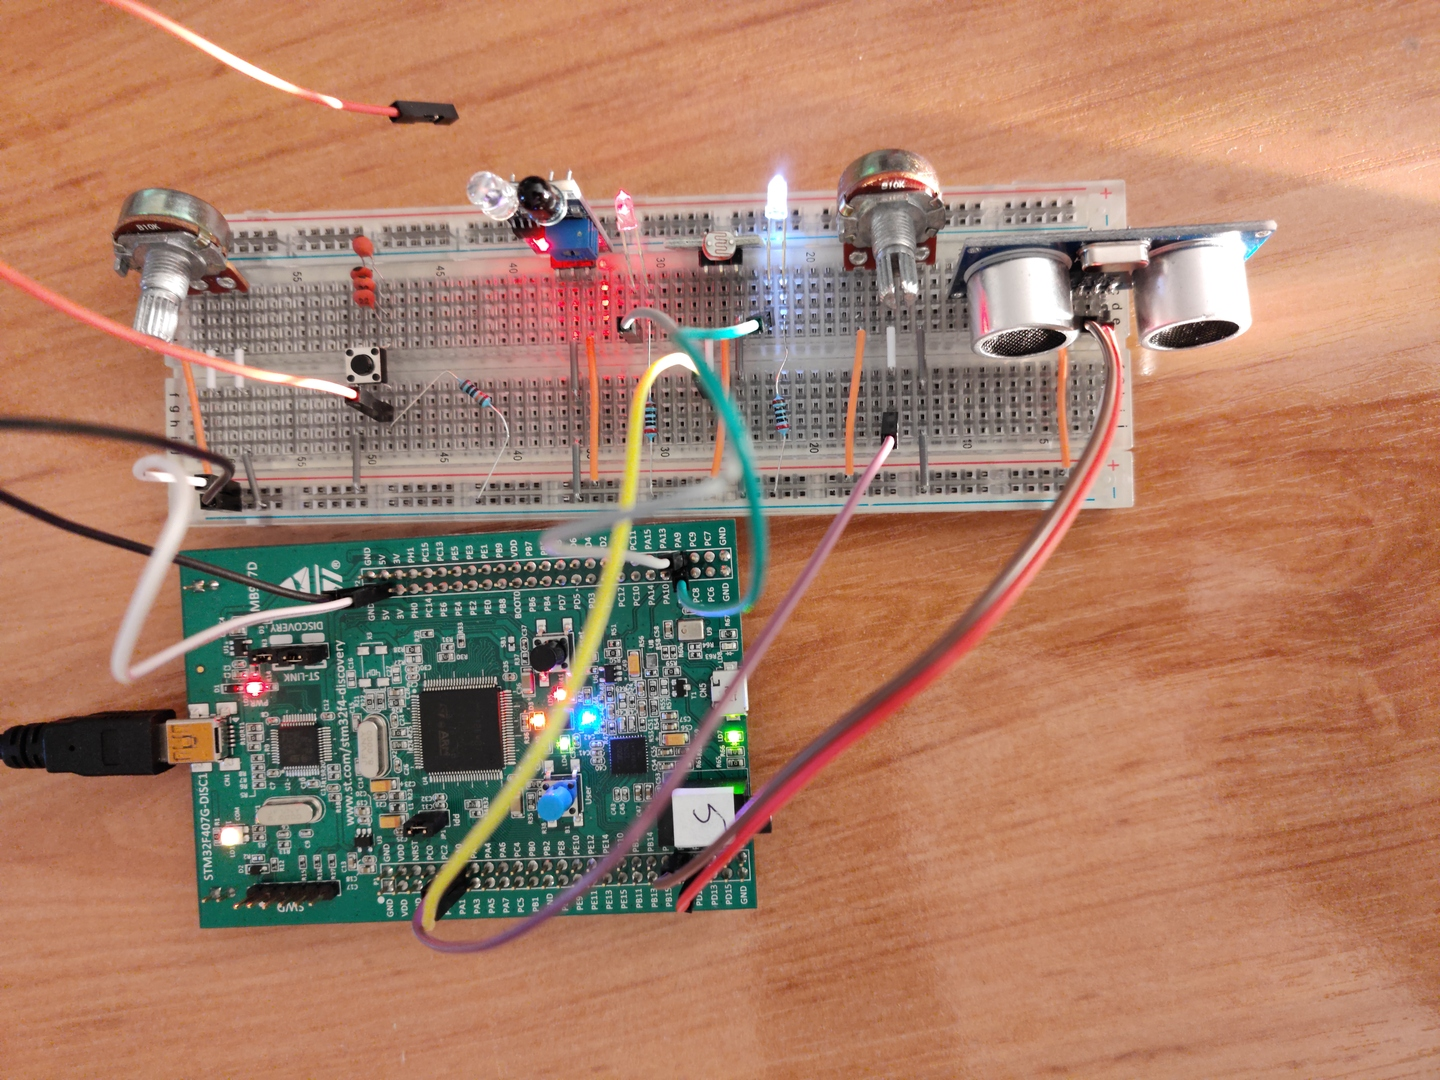
\includegraphics[width=\linewidth]{pictures/final-design.lq.jpg}
  \caption{Diseño final del circuito montado sobre una \textit{protoboard}.}
  \label{fig:final-design}
\end{figure}

Como se puede ver en la figura anterior, todo el circuito (de los dos nodos)
se ha podido montar sobre la misma placa de desarrollo: se pueden apreciar los
dos potenciómetros (volante y acelerador), el sensor de presencia para el agarre
del volante, LDR para luz ambiental, múltiples LEDs para mostrar señales, etc.

Con el código implementado se ha conseguido que las tareas funcionen como se esperaban
y que se puedan realizar algunas comunicaciones mediante el CANBus. Sin embargo, la
falta de tiempo (e inexperiencia del equipo) durante el desarrollo del proyecto ha
dejado \textit{bugs} sin resolver y el código no está todo lo depurado que
convendría para un sistema en tiempo real.

Por otra parte, y en estrecha relación con lo mencionado anteriormente, solo se
han podido implementar dos nodos, teniendo que postergar el desarrollo del nodo
\textit{display} para otro momento.

Finalmente, se asume que el sistema es planificable ya que los accesos a CPU y
recursos no son tan grandes como para que alguna tarea saliese no planificable.
Sin embargo, sería interesante poder realizar observaciones y mediciones sobre
un prototipo en avanzado estado de desarrollo para extraer el WCET $C_i$ de
cada tarea, realizar el RTA (\textit{Response Time Analysis}) y verificar que
efectivamente el sistema es planificable o, en otro caso, realizar los ajustes
pertinentes para que lo sea.
\section{Aclaraciones}
\begin{itemize}
  \item En los códigos \ref{lst:speedtask} y \ref{lst:lightstask}, el mapeo se realiza con valores
        de entrada $\left[0, 255\right]$ porque el ADC de la placa
        es de 8 bits, por lo que su resolución máxima es 255.
  \item En diversos códigos (como \ref{lst:distancetask} o \ref{lst:braketask}) se
        utilizan eventos para la sincronización de tareas entre sí. Los eventos
        aparecen en la documentación estándar de FreeRTOS y constituyen un mecanismo
        muy sencillo y eficiente que respeta el tiempo real para bloquear y desbloquear
        tareas sin necesidad de programar la lógica subyacente. Un evento, en esencia,
        se conforma de $1 \dots n$ procesos que esperan y, en principio, un único proceso
        $k$ que ``produce'' el evento. En ese instante, aquellas tareas que estaban
        esperando al evento se desbloquean y prosiguen con su ejecución; mientras tanto,
        el proceso $k$ reiniciaría el evento de forma que nuevas tareas pueden esperar
        a que se produzca.

        De esta manera, una tarea esporádica estaría esperando a que un evento se
        produzca y existiría una tarea periódica activadora la cual indicaría
        mediante dicho evento a la tarea esporádica que se tiene que ejecutar.
  \item En el código \ref{lst:wheel-task} se esperan 13 iteraciones que equivalen a un
        tiempo de $\numprint[s]{5.2}$ (en lugar de los $\numprint[s]{5}$ pedidos). Esto
        es debido a que el periodo no es múltiplo, por lo que se comete un error
        ``a la alta'' en lugar de ``a la baja''.
  \item Los ficheros \texttt{lock.h/.c} permiten trabajar con semáforos definidos de
        forma estática en lugar de forma dinámica (código \ref{lst:lock_c}). Sin embargo,
        para poder aprovechar dicha funcionalidad es necesario habilitar en el fichero
        \texttt{FreeRTOSConfig.h} la macro:
        \begin{center}
            \lstinline[style=C]!#define configSUPPORT_STATIC_ALLOCATION 1!
        \end{center}
        con un valor `1'. En otro caso, aunque se pase un parámetro válido, no se usará
        dicha funcionalidad.
  \item El pitido no se ha implementado a nivel de código ya que no venía especificado
        en los distintos diagramas a qué pin habría que conectarlo ni la lógica de
        control a usar para que funcionase con cierta intensidad.
  \item En el código \ref{lst:canbustasks} se han implementado dos tareas esporádicas
        para la gestión de los mensajes del CANBus porque dicho dispositivo recibe 
        mensajes desde una rutina de interrupción. Como se quieren
        actualizar variables las cuales utilizan un \texttt{lock} internamente, se
        deriva su gestión a un par de tareas esporádicas cuya única finalidad es la
        de actualizar el valor de los objetos protegidos.
  \item En los códigos \ref{lst:can_h} y \ref{lst:can_c}, como son en apariencia iguales
        para ambos nodos, es necesario definir una macro para que la versión del CANBus
        se adapte a la placa en que se ejecuta. De esta forma, en el nodo 2 habría que
        definir en alguna cabecera (se sugiere \texttt{FreeRTOSConfig.h}) la macro:
        \begin{center}
              \lstinline[style=C]!#define NODE_2!
        \end{center}
  \item En el código \ref{lst:riskstask} no se ha implementado la parte de interacción
        con el freno ya que la tarea \texttt{Cálculo distancia} (código \ref{lst:distancetask})
        se encarga individualmente de accionar el freno según la distancia de seguridad
        y una intensidad predefinida. Además, en las diapositivas de la especificación
        no se menciona esta comunicación con el nodo 1, por lo que se ha asumido que
        el verdadero encargado de accionar el freno es el nodo 1.
\end{itemize}
\section{Glosario}
\begin{center}
  \textit{FreeRTOS, SysML, paralelismo, sincronización, C, desarrollo colaborativo, planificación,
  comunicación hardware, gestión de recursos, CANBus.}
\end{center}

\newpage

\appendix
\section{Código fuente común}
\label{anx:common-code}
\subsection{Cabeceras de código}
\lstinputlisting[style=C,caption={Cabecera con funciones de utilidad.},label={lst:utils_h}]{source-code/node1/Inc/utils.h}
\lstinputlisting[style=C,caption={Cabecera de la librería CANBus.},label={lst:can_h}]{source-code/node1/Inc/can.h}
\lstinputlisting[style=C,caption={Cabecera de la librería \texttt{lock}.},label={lst:lock_h}]{source-code/node1/Inc/lock.h}
\subsection{Cuerpo del código}
\lstinputlisting[style=C,caption={Cuerpo de las funciones de utilidad.},label={lst:utils_c}]{source-code/node1/Src/utils.c}
\lstinputlisting[style=C,caption={Cuerpo de la librería CANBus.},label={lst:can_c}]{source-code/node1/Src/can.c}
\lstinputlisting[style=C,caption={Cuerpo de la librería \texttt{lock}.},label={lst:lock_c}]{source-code/node1/Src/lock.c}

\section{Código fuente nodo 1}
\subsection{Cabeceras de código}
\lstinputlisting[style=C,caption={Cabecera del objeto protegido \texttt{speed}.},label={lst:speed_h}]{source-code/node1/Inc/speed.h}
\lstinputlisting[style=C,caption={Cabecera del controlador de ultrasonidos.},label={lst:uss_h}]{source-code/node1/Inc/uss.h}
\lstinputlisting[style=C,caption={Cabecera del objeto protegido \texttt{distance}.},label={lst:distance_h}]{source-code/node1/Inc/distance.h}
\lstinputlisting[style=C,caption={Cabecera del objeto protegido \texttt{brake}.},label={lst:brake_h}]{source-code/node1/Inc/brake.h}
\subsection{Cuerpo del código}
\lstinputlisting[style=C,caption={Cuerpo del objeto protegido \texttt{speed}.},label={lst:speed_c}]{source-code/node1/Src/speed.c}
\lstinputlisting[style=C,caption={Cuerpo del controlador de ultrasonidos.},label={lst:uss_c}]{source-code/node1/Src/uss.c}
\lstinputlisting[style=C,caption={Cuerpo del objeto protegido \texttt{distance}.},label={lst:distance_c}]{source-code/node1/Src/distance.c}
\lstinputlisting[style=C,caption={Cuerpo del objeto protegido \texttt{brake}.},label={lst:brake_c}]{source-code/node1/Src/brake.c}

\section{Código fuente nodo 2}
\subsection{Cabeceras de código}
\lstinputlisting[style=C,caption={Cabecera del objeto protegido \texttt{mode}.},label={lst:mode_h}]{source-code/node2/Inc/modes.h}
\lstinputlisting[style=C,caption={Cabecera del objeto protegido \texttt{symptoms}.},label={lst:symptoms_h}]{source-code/node2/Inc/symptoms.h}
\lstinputlisting[style=C,caption={Cabecera del objeto protegido \texttt{node1}.},label={lst:node1_h}]{source-code/node2/Inc/node1.h}
\subsection{Cuerpo del código}
\lstinputlisting[style=C,caption={Cuerpo del objeto protegido \texttt{mode}.},label={lst:mode_c}]{source-code/node2/Src/modes.c}
\lstinputlisting[style=C,caption={Cuerpo del objeto protegido \texttt{symptoms}.},label={lst:symptoms_c}]{source-code/node2/Src/symptoms.c}
\lstinputlisting[style=C,caption={Cuerpo del objeto protegido \texttt{node1}.},label={lst:node1_c}]{source-code/node2/Src/node1.c}

\end{document}